\documentclass[12pt]{article}
\linespread{2}
\usepackage{times}
\usepackage{pgfplots}
\usepackage[dvipsnames]{xcolor}
\pgfplotsset{compat = newest}
\usetikzlibrary{positioning, arrows.meta}
\usepgfplotslibrary{fillbetween}
\usepackage{amsmath}
           \begin{document} 
                 \begin{center}
                       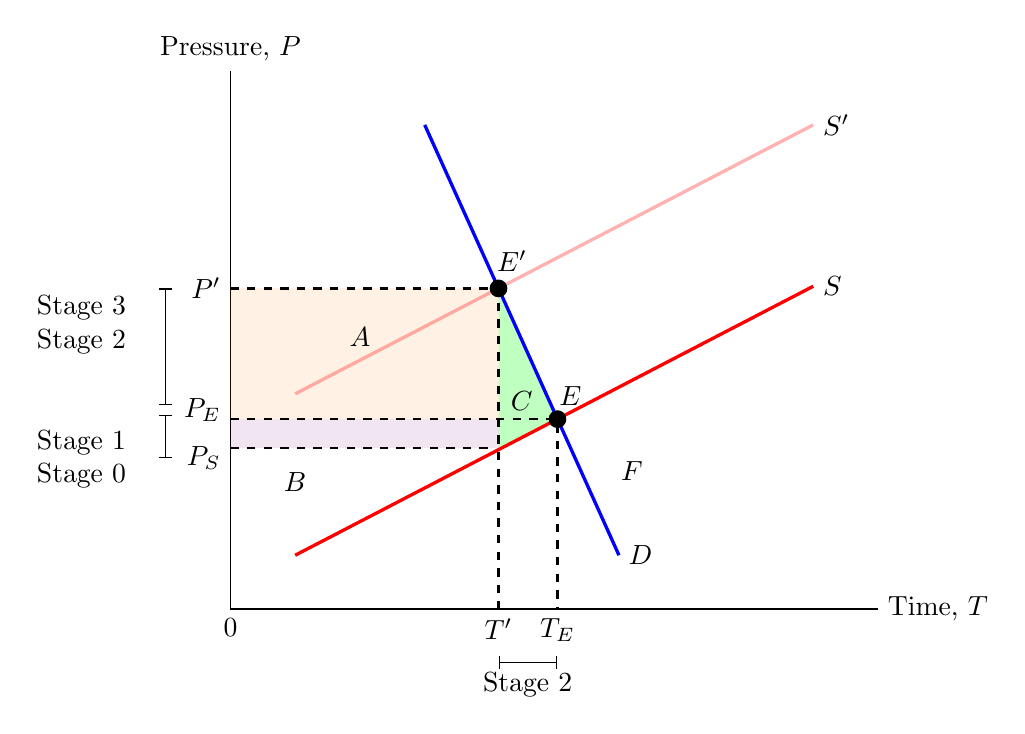
\begin{tikzpicture}
                             \begin{axis}[
                                          scale = 1.2,
                                          xmin = 0, xmax = 10,
                                          ymin = 0, ymax = 10,
                                          axis lines* = left,
                                          xtick = {0}, ytick = \empty,
                                          clip = false,
]


% Colouring areas
                    \fill[orange, opacity = 0.1] (0, 3.53) -- (4.14, 3.53) -- (4.14,
                          5.96) -- (0, 5.96);
                    \fill[violet, opacity = 0.1] (0, 3.53) -- (4.14, 3.53) -- (4.14,
                          3) -- (0, 3);
                    \fill[green, opacity = 0.25] (4.14, 3.53)-- (5.05, 3.53) -- (4.14,
                          5.96);
                    \fill[green, opacity = 0.25] (4.14, 3)-- (5.05, 3.53) -- (4.14,
                          3.53);


% Supply and demand curves
                      \addplot[color = blue, very thick] coordinates {(3,9) (6,1)};
                      \addplot[color = red, very thick] coordinates {(1,1) (9,6)};
                      \addplot[color = red, opacity = 0.3, very thick] coordinates
                              {(1,4) (9,9)};
                              
% Dashed lines
                      \addplot[color = black, dashed, thick] coordinates {(0, 5.96)
                               (4.14, 5.96) (4.14, 0)};
                      \addplot[color = black, dashed, thick] coordinates {(0, 3.53)
                               (5.05, 3.53) (5.05, 0)};
                      \addplot[color = black, dashed, thick] coordinates {(0, 3) (4.1,
                                3)};


% Coordinate points
                      \addplot[color = black, mark = *, only marks, mark size = 3pt]
                            coordinates {(4.14, 5.96) (5.05, 3.53)};


% Labels
                  \node [right] at (current axis.right of origin){Time, $T$};
                  \node [above] at (current axis.above origin) {Pressure, $P$};
                  \node [above] at (5.25, 3.6) {$E$};
                  \node [above] at (4.35, 6.1) {$E^\prime$};
                  \node [right] at (6, 1) {$D$};
                  \node [right] at (9, 6) {$S$};
                  \node [right] at (9, 9) {$S^\prime$};
                  \node [left] at (0, 3.7) {$P_E$};
                  \node [left] at (0, 2.8) {$P_S$};
                  \node [left] at (0, 5.96) {$P^\prime$};
                  \node [below] at (5.05, 0) {$T_E$};
                  \node [below] at (4.14, 0) {$T^\prime$};
                  \node [above] at (2, 4.7) {$A$};
                  \node [above] at (1, 2) {$B$};
                  \node [above] at (4.5, 3.5) {$C$};
                  \node [above] at (6.2, 2.2) {$F$};


% Arrows

               \draw[|-|] (-1, 5.96) to (-1, 3.8);
               \draw[|-|] (4.14, -1) to (5.05, -1);
               \node [below] at (4.59, -1) {{Stage 2}};
               \node [below, align = left] at (-2.3, 6) {Stage 3 \\ Stage 2};
               \draw[|-|] (-1, 3.6) to (-1, 2.8);
               \node [below, align = left] at (-2.3, 3.5) {Stage 1 \\ Stage 0};


                         \end{axis}
                   \end{tikzpicture}
            \end{center}


                \textbf{Figure 16 }
  \end{document} 